\section{Durchführung und Aufbau}
\label{sec:Aufbau}
Der Versuchsaufbau besteht aus einer Röntgenröhre (3), einem drehbar gelagertem
Kristall (2) und einem verstellbaren Geiger-Müller-Zählrohr (1),
gemäß Abbildung \ref{fig:röntgen}.
\\
Zunächst wird die Braggbedingung für einen Lithiumflourid(LiF) Kristall
überprüft. Dafür wird der Kristallwinkel auf $\SI{14}{\degree}$
festgestellt und mit dem Geiger-Müller-Zählrohr wird die Intensität in
$\SI{0.1}{\degree}$-Schritten gemessen, indem die Impulse
$\SI{20}{\second}$ je Winkel gemessen werden.
\\
Danach wird das Emissionsspektrum einer Kupfer-Röntgenröhre in 2:1-Winkel-Kopplung
von Kristall und Zählrohr aufgenommen, mit je $\SI{5}{\second}$ Integrationszeit.
\\
Das Absorptionsspektrum wird für 5 verschiedene Elemente genommen:\\
Zink(Z=30), Zirkonium(Z=40), Strontium(Z=38), Brom(Z=35) und Quecksilber(Z=80).\\
Um das Absorptionsspektrum zu erhalten wird der jeweilige Absorber auf dem
Geiger-Müller-Zählrohr befestigt und es wird wieder in einem geeigneten
Winkelbereich das Spektrum aufgenommen.

\begin{figure}
    \centering
    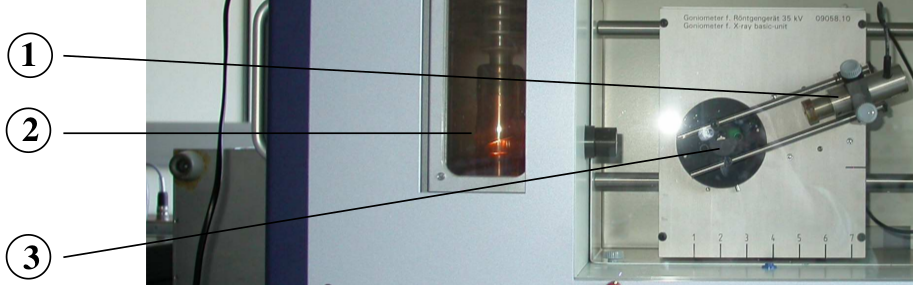
\includegraphics[width=11cm]{content/roentgenklein.png}
    \caption{Aufbau der verwendeten Röntgenröhre. \cite{Anleitung}}
    \label{fig:röntgen}
\end{figure}
